\documentclass[
  10pt
%, handout
]{beamer}
%\setbeameroption{show notes on second screen}

% TODO: What is this for?
\usepackage{pgfpages}
\usepackage{pdfpages}

% Use T1 Font encoding to support more glyphs
\usepackage[T1]{fontenc}

% Number sections in table of contents
\setbeamertemplate{section in toc}[sections numbered]
% Hide subsections in table of contents
\setcounter{tocdepth}{1}

\usetheme{metropolis}

% Also number pages in appendix
\usepackage{appendixnumberbeamer}

% Nicer tables
\usepackage{booktabs}

% foo
\setbeamertemplate{caption}{\raggedright\insertcaption\par}

\usepackage[normalem]{ulem}

\usepackage[scale=2]{ccicons}

\usepackage{pgfplots}
\usepgfplotslibrary{dateplot}

\usepackage{xspace}
\newcommand{\themename}{\textbf{\textsc{metropolis}}\xspace}

\usepackage{graphicx}
\usepackage{listings}

\usepackage{lmodern}

\usepackage{eurosym}
\usepackage{amsmath, amssymb}
\usepackage[binary-units=true]{siunitx}
\DeclareSIUnit{\EUR}{\text{\euro}}

\usepackage{xcolor}
\newcommand\crule[3][black]{\textcolor{#1}{\rule{#2}{#3}}}

\newcommand{\tinycite}[1]{\tiny{(\cite{#1})}}
%\newcommand{\tinycite}[1]{foo}

\title{Porting EDK2 UEFI to RISC-V}
\subtitle{Open Source Firmware, BMC and Bootloader devroom}
\date{February 6, FOSDEM 2021}
\author{Daniel Schaefer}

\begin{document}

\maketitle

\begin{frame}{Agenda}
  \begin{itemize}
    \item About us
    \item History of booting on RISC-V
      % Explain how RISC-V was initially booted,
      % How U-Boot has become the default and how Edk2 can possibly become the second default
      % Also mention oreboot as a recent mature implementation
    \item UEFI on RISC-V
    \item History of the implementation
      % Explain the history, how Abner got started in 2016
      % how he implemented a PC-AT version of RISC-V in qemu and abandoned it
      % How OpenSBI revived it
      % How we upstreamed it in 2020
      % And how we're currently working on and upstreaming Linux support
    \item Architecture of EDK2 on RISC-V
      % Self-explaining
    \item Booting to Linux
      % Explain the steps that were required to make Linux boot
      % and show the details
    \item Full Details of Booting on Hifive Unleashed and QEMU
      % Quickly go through all of the details to give an walkthrough from beginning to end
    \item Demo booting to Linux
    \item Goals for the future of this implementation
    \item Vision for the future
  \end{itemize}
  %\tableofcontents
\end{frame}

\begin{frame}{About us}
  \begin{itemize}
    \item UEFI Firmware Engineers for ProLiant Servers at HPE
    \item Great learning opportunity: Changes required in entire  UEFI boot flow
    % TODO: Maybe
    % From SEC through to starting the bootloader (EFISTUB)
  \end{itemize}

  \vfill

  \begin{columns}
    \column{0.5\textwidth}
    \begin{figure}[h]
      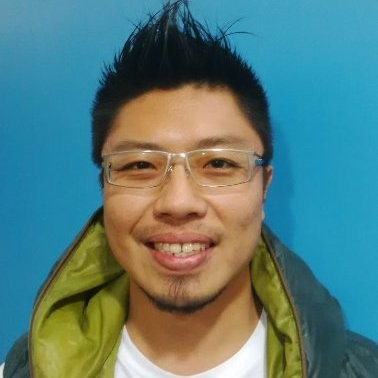
\includegraphics[width=0.3\textwidth]{resources/abner.jpg}
      \caption{Abner Chang}
    \end{figure}
    \begin{itemize}
      \item Working on UEFI for many years
      \item Started the project 
    \end{itemize}

    \column{0.5\textwidth}
    \begin{figure}[h]
      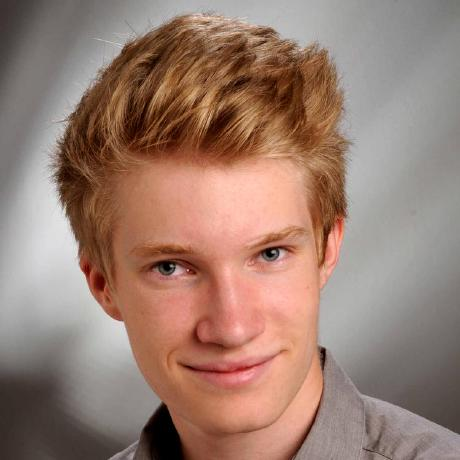
\includegraphics[width=0.3\textwidth]{resources/daniel.jpg}
      \caption{Daniel Schaefer}
    \end{figure}

    \begin{itemize}
      \item Graduated last year
      \item First full-time UEFI project
    \end{itemize}
  \end{columns}
\end{frame}

\begin{frame}{Disclaimer}
  % We did the work mostly at work as a side project
  % But
\end{frame}

\begin{frame}{EDK2}
  \centering
  
\includegraphics[width=0.3\textwidth]{resources/tianocore-logo.png}

  \vfill

  \begin{itemize}
    \item UEFI is only an interface specification
    \item EDK2 is the reference implementation of UEFI
    \item Initially developed for Itanium
    \item Now mainstream for x86\_64
    \item ARM % Aarch32 since 2009, Aarch64 since 2013, part of BBR standards...
  \end{itemize}
\end{frame}

\begin{frame}{RISC-V}
  \centering
  
\includegraphics[width=0.3\textwidth]{resources/riscv-logo.png}

  \vfill

  \begin{itemize}
    \item "Free and Open RISC Instruction Set Architecture"
    % Implementations aren't required to be open
    \item Tries to be simple and legacy-free
    \item Three privilege modes (\textbf{M}achine, \textbf{S}upervisor, \textbf{U}ser)
      % Implementations are only required to provide Machine
      % There's now also, optionally, Hypervisor
    \item Similar to x86 boot starts without MMU in Machine mode
      % Firmare and OS have to enable MMU and transition to S&M
    \item FW can stay resident after boot and be called by higher layers \\
          Like x86's SMM but with well defined interface like Itanium's PAL/SAL \\
          $\rightarrow$ Supervisor Binary Interface (SBI)
  \end{itemize}
\end{frame}

% TODO: Maybe compare diagrams of SBI and SAL
% TODO: Maybe add a slide of SBI OpenSBI

% We use OpenSBI as an SBI implementation and helper library
% Differently than U-Boot and coreboot we don't use it to load EDK2 or as a payload
% 
% Calling SBI works the same way as userspace makes kernel calls (syscall or ecall in RISC-V)

\begin{frame}{History of booting on RISC-V}
  \begin{itemize}
    \item 201? BBL % Berkeley Boot Loader, original research bootloader
    \item 2016 EDK2 Prototype with QEMU RISC-V PC/AT board % [4]
    \item 201? U-Boot+OpenSBI
    \item 2020 EDK2+OpenSBI Upstream
    \item 201? U-Boot+OpenSBI with UEFI interface

    \item 20?? Coreboot
    \item 20?? Oreboot
  \end{itemize}
\end{frame}

\begin{frame}{Timeline of this implementation}
  \begin{itemize}
    \item 2015: Started by Abner
    \item 2015: Started by Abner
  \end{itemize}
\end{frame}

% Think about how to integrate Abner's diagram

\begin{frame}{Details}
% -------
Example based on Hifive Unleashed (U540) and equivalent sifive\_u QEMU model

Starts running in M-Mode

ZSBL (zero stage bootloader)
  Embedded in mask ROM or hardcoded in QEMU source
  Jumps to predefined address, so we need to put our FW there

SEC
  - Starts in ASM
  - Set up scratch register
  - Set up stack in temporary RAM
  - Set up trap handler
    - Check privilege mode
    - Save registers
    - Call OpenSBI's trap handler
    - Restore registers
  - Call SecCore C function with hartid (mhartid) scratch pointer (mscratch)
    - Save some machine information from registers in private space in scratch space
      - march
      - Also OpenSBI function to switch mode
  - Initialize OpenSBI passing it scratch pointer with
    - device tree % OpenSBI wants to fix it up in sbi_init, not sure if that's still necessary
    - next mode (M-Mode still)
    - platform specific functions
      - PLIC, CLIC config
      - PMP config to make SEC and PEI code rx only, adapted from OpenSBI source file
  - Initialize possibly other harts and stall them, only one hart will continue to boot
  - Register custom SBI calls
    - To get mscratch for current or arbitrary hart
    - We don't want to call the library after SEC, so we use SBI ecalls
    - TODO: Should deregister this later because it's only supposed to be used by UEFI
    % I think (Open)SBI doesn't yet have a way to do this
  - Find PEI entrypoint in boot firmware volume (hardcoded offset)
  - Switch to S-Mode
  - Enable identity mapped MMU
  - Jump to PEI and switch to S mode
    - Originally we used M-Mode still but it's good to reduce privileges early on and enable MMU

PEI
  - Pass it information about location and size of:
    - boot firmware volume
    - temporary ram
    - stack
  - "Discover" RAM and tell UEFI about it (hardcoded)
  - Take device tree from scratch space and store in HOB
  - Discover some more processor features and save it, later add it to SMBIOS
  - Build new stack in actual RAM
  - Switch stack and execute DxeIpl (initial program loader)
  - Previously this was where we switched to S-Mode and initialize OpenSBI
    But we want to initialize OpenSBI earlier and have less privileges earlier

DXE
  - Install timer protocol
    - Also install interrupt handler for timer interrupt in S-Mode
  - Install RuntimeServices
  - Install SMBIOS tables using information from PEI
   - Type 4 (CPU)
   - Type 7 (Caches)
   - Type 44 (Additional CPU information) New
     https://github.com/riscv/riscv-smbios/
  - Take device tree from HOB and store in EFI System Configuration Table
    - Also put the boot hart-id in device tree, as required by Linux

BDS (UEFI Shell)
  - For booting linux I embedded the EFISTUB kernel and initrd in the flash image
    With a command on the shell you can load it into ram and turn it into a ramdisk
  - Load initrd into with `initrd` command and install protocol on fixed device path

EFISTUB (Implemented by Atish, tested and finalized in cooperation with us)
  - Take device tree from EFI System Configuration Table
  - Call LoadFile2 on fixed device path to extract initrd
  - Execute kernel proper
    - Disable MMU
    - `jump\_kernel(hartid, fdt);`


% -------
\end{frame}

\begin{frame}{Demo}

\end{frame}

\begin{frame}{UEFI on RISC-V}
  % Explain what this is all about
  % That we ported the reference implementation of UEFI, namely EDK2 to RISC-V
  % Mhh forgot what else

  % 
\end{frame}

% TODO: Use proper checkmark and x symbol
\begin{frame}{Status - EDK2}
  \begin{itemize}
    \item y UEFI Shell
    \item y UEFI Applications (e.g. bootloader)
    \item y Booting Linux via EFISTUB
  \end{itemize}
\end{frame}

\begin{frame}{Status - Platforms}
  \begin{center}
    \begin{tabular}{|l|l|l|l|}
      \hline
      Platform Name     & UEFI Shell & Linux \\
      \hline
      HiFive Unleashed  & Yes        & Yes \\
      QEMU sifive\_u    & Yes        & Yes \\
      % VC707
      Freedom U500 FPGA & Yes        & N/A \\
      % Very important! Will help us get proper disk and 
      QEMU virt         & N/A        & N/A \\
      % We have the board, just haven't gotten around to porting it yet
      Andes AE350       & N/A        & N/A \\
      % Registered for early dev board to port until general availability
      BeagleV           & N/A        & N/A \\
      \hline
    \end{tabular}
    % See our status page
  \end{center}
\end{frame}

\begin{frame}{Status - Overall}
  \begin{itemize}
    \item UEFI specification amended
    \item SMBIOS specification amended
    \item EDK2 port merged upstream
    % Haven't tested it on EDK2 yet, but works on U-Boot
    \item UEFI Self Certification Test ported, patches need cleanup
    \item Linux EFISTUB ported by Atish, merged in 5.10
  \end{itemize}
\end{frame}

\begin{frame}{Goals}
  \begin{itemize}
    % OpenSBI 0.9 has support for that
    \item Implement \textit{ResetSystem} Runtime Service with SBI (WIP) % [2]
    \item Upstream changes for booting Linux (FDT fixup and storing)
    \item SD card driver for Hifive Unleashed
    \item Implement new relocation types by newer GNU toolchains % [1]
    \item Build "OVMF" for QEMU's virt platform with VirtIO drivers \\
          $\rightarrow$ Add boot tests to EDK2 CI \\
          $\rightarrow$ Boot with actual disk! \\
    \item Port to BeagleV when it arrives
  \end{itemize}
\end{frame}

\begin{frame}{How to help}
  \begin{itemize}
    % TODO: What's required for that?
    \item Port to new boards, talk to us
    \item Check out the issues on the repo
  \end{itemize}
\end{frame}

\begin{frame}{Vision for the future}
  \begin{itemize}
    \item Make RISC-V boot like rest of industry \\
          U-boot for embedded, UEFI for consumer and server
          % TODO: Not sure about coreboot and LinuxBoot
    \item Follow in ARM's footsteps to \textit{make booting boring}
          % Perhaps we need something like SBBR, EBBR, ...
    \item Encourage discussion about desktops and servers
          % Some companies have started developing powerful chips
  \end{itemize}
\end{frame}

\begin{frame}{Thanks}
  Question Time!

  Daniel Schaefer <git@danielschaefer.me>
\end{frame}

% TODO:
% - https://fosdem.org/2021/schedule/event/firmware_uor/
% - Upload slides

\begin{frame}{References}
% # Sources
% - Itanium SAL/PAL: https://www.csee.umbc.edu/portal/help/architecture/24535901.pdf
% - BBL: https://www.lowrisc.org/docs/build-berkeley-boot-loader/
% - U-Boot
% - Coreboot
% - Oreboot
% - QEMU
% - https://github.com/riscv/riscv-sbi-doc
% - https://github.com/riscv/riscv-uefi-edk2-docs
% - https://github.com/riscv/riscv-edk2
% - https://github.com/riscv/riscv-edk2-platforms
% - [1] https://github.com/riscv/riscv-edk2/issues/3
% - [2] https://github.com/riscv/riscv-sbi-doc/commit/2f101582210b17a61e2f2bd356a01c6bda467ed0
% - [3] https://beagleboard.org/beaglev
% - [4] Abner and Dong's presentation from 2016: https://www.youtube.com/watch?v=9c73WHduovs

\end{frame}

\begin{frame}{Glossary}
% UEFI
% EDK2
% Tianocore
% RISC-V
% MMU
% SBI
% Itanium
% SBI
% PAL
% SAL
% RISC
\end{frame}

\end{document}
